\documentclass[a4paper]{article}
\usepackage[T1]{fontenc}
\usepackage[margin=1in]{geometry}
\usepackage{listings}
\usepackage{xcolor}
\usepackage{courier}
\usepackage{graphicx}
\usepackage{hyperref}
\usepackage{sidecap}
\usepackage{wrapfig}
\usepackage{subfig}
\usepackage{float}
\renewcommand{\figurename}{Rysunek}

\lstdefinestyle{sharpc}{language=[Sharp]C, frame=lr, rulecolor=\color{blue!80!black}}

\title{Cechy sygnału audio w dziedzinie czasu\\
\large Projekt nr 1 - Analiza i Przetwarzanie Dźwięku\\ 
\small \url{https://github.com/szymon159/sound-analysis}}
\date{}
\author{Szymon Stasiak}

\begin{document}
  \maketitle

\section{Opis aplikacji}
Projekt stworzony został w .NET Framework, z warstwą prezentacji powstałą w Windows Forms i interfejsem w języku angielskim.\\
W celu uproszczenia i zoptymalizowania wczytywania i parsowania plików (\textit{*.wav} oraz \textit{*.mp3}), projekt korzysta także z jednej dodatkowej paczki nugetowej - NAudio.\\
Jako nagrania testowe posłużyły udostępnione transkrypcje (\textit{Rysunki 2 i 3}), a ponadto: utwór \textit{Portier!} Taco Hemingwaya (jako przykład rozmowy z tłem muzycznym) - \textit{Rysunki 1, 4, 5}, fragment przemówienia Baracka Obamy (jako przykład mowy, pobrany ze strony \url{http://soundbible.com/}) - \textit{Rysunek 6} oraz fragment utworu \textit{Adventure} stworzony przez Bensound (jako przykład muzyki instrumentalnej, udostępniony za darmo na stronie \url{https://www.bensound.com/royalty-free-music/)} - \textit{Rysunek 7}.
\subsection{Głowne okno programu}
\begin{figure}[H]
  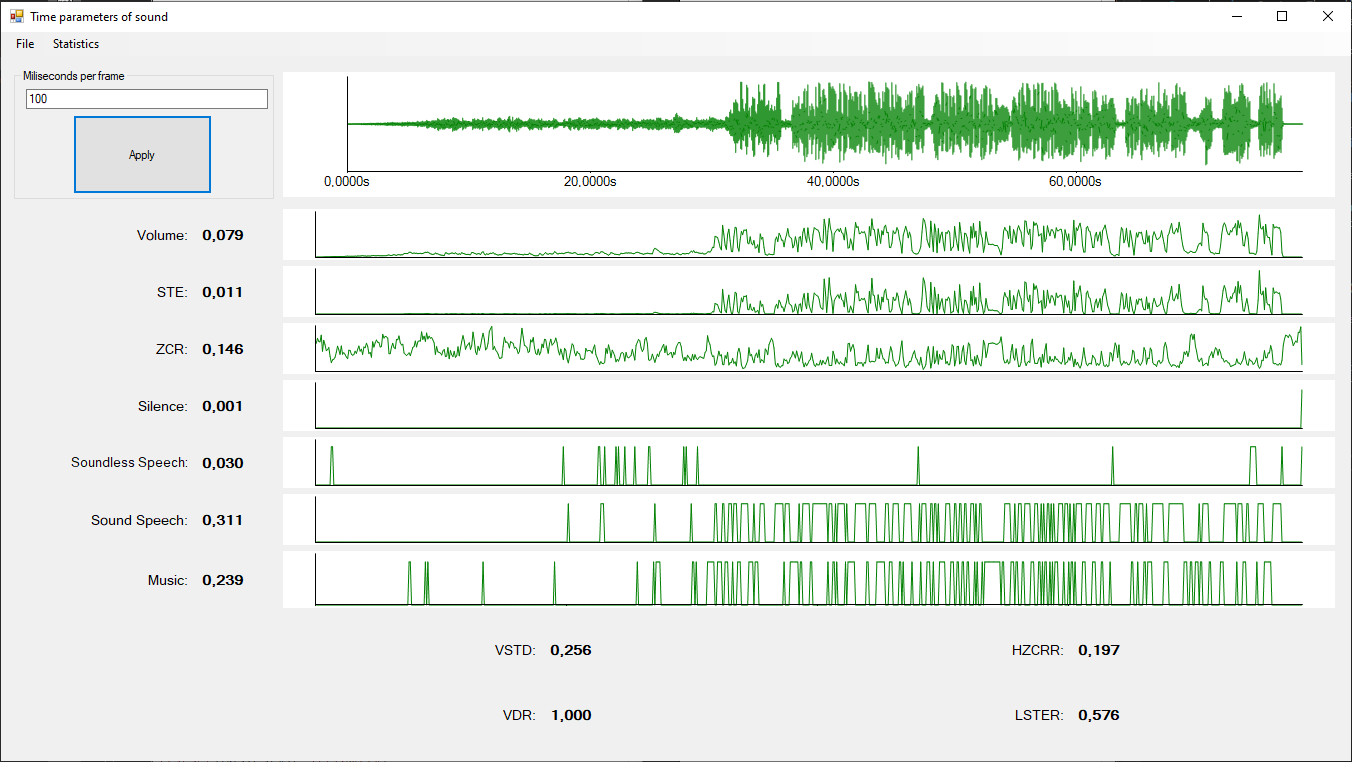
\includegraphics[width=\linewidth]{images/01interface.png}
  \caption{Interfejs programu}
\end{figure}
Parametry obok wykresów oznaczają średnią z wartości dla wszystkich ramek nagrania.

\subsection{Statystyki}
Przycisk \textit{Statistics} w menu na górze okna otwiera menu kontekstowe pozwalające dla każdego dostępnego typu statystyki (wspierane: \textit{cisza}, \textit{mowa bezdźwięczna}, \textit{mowa dźwięczna}, \textit{muzyka}) wyświetlić lub wyeksportować statystki.\\
W przypadku decyzji o wyświetleniu, w pojawiającym się okienku modalnym, znajduje się lista interwałów, w których dane zjawisko zostało zaobserwowane oraz ich długość.\\
W przypadku wybrania eksportu, pojawia się okno zapisu pliku. W zapisanym pliku \textit{*.csv} każda linia oznacza jeden interwał. Numer interwału, czas początku, czas końca i długość są oddzielone przecinkiem. Dodatkowo pierwsza linia zawiera opisy kolumn.

\section{Opis metod}
\subsection{Cechy na poziomie ramki (Frame-level)}
Ilość ramek wyliczana jest na podstawie podanej wartości milisekund na ramkę (\textit{Miliseconds per frame}, lewy górny róg) oraz pobranej przy wczytywaniu pliku częstotliwości próbkowania.\\
Na wszystkich wykresach wartość dla ramki zaznaczona jest w jej środku. W przypadku nierównego podziału, ostatnia ramka może być dużo krótsza niż pozostałe (jednak punkt wciąż zaznaczony jest w jej środku).\\
We wszystkich wzorach z tego rozdziału zachowane zostało następujące znaczenie symbol: \textit{$n$} - kolejny indeks ramki, \textit{$M$} - długość ramki w próbkach, \textit{$s_n(i)$} - amplituda i-tej próbki w n-tej ramce, \textit{$sign(x)$} - funkcja signum.\\
Ponadto poniższe omówienie wszystkich cech może zawierać odwołania do przykładowych nagrań (zarówno nieznormalizowanego jak i znormalizowanego). W celu uproszczenia odbioru, \textit{Rysunek 2} oraz \textit{Rysunek 3} prezentują jedno przykładowe nagranie w obu tych wariantach.
\begin{figure}[H]
  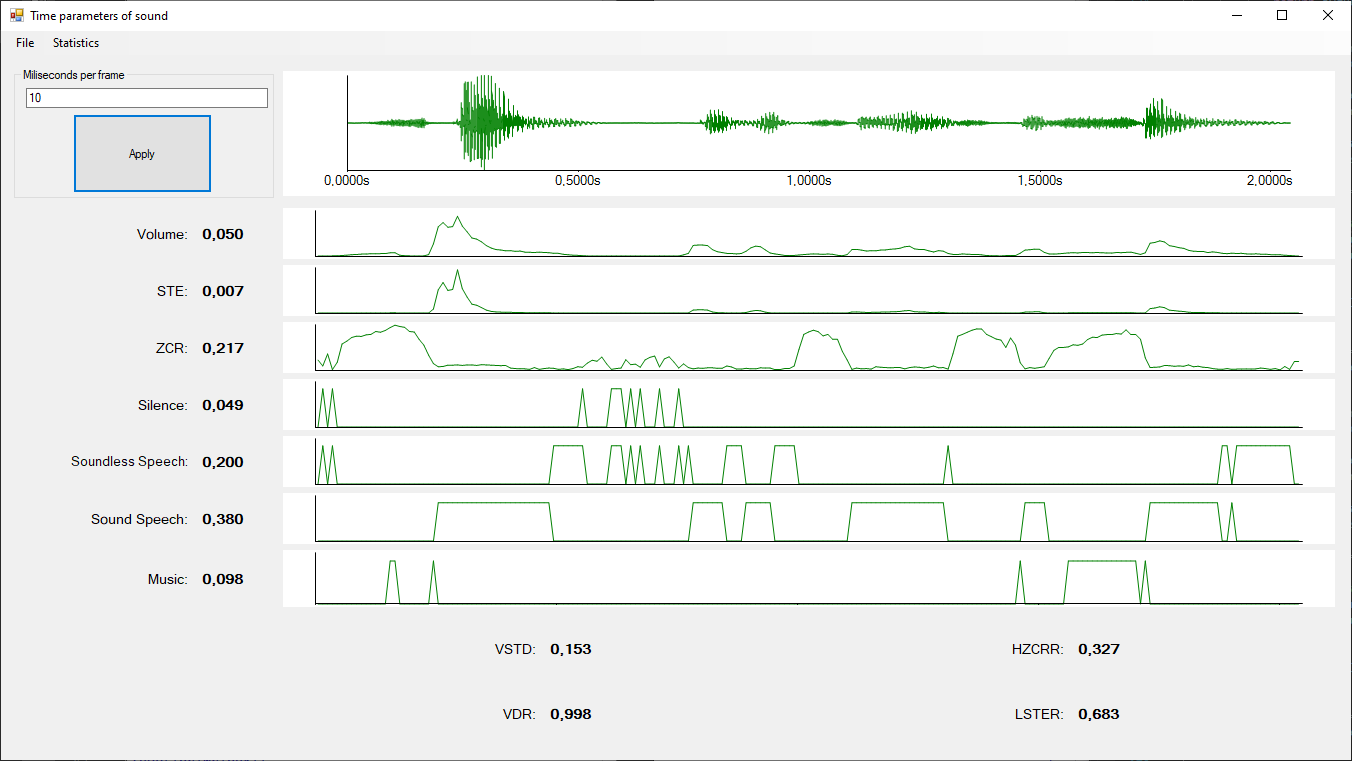
\includegraphics[width=\linewidth]{images/02notnormalized.png}
  \caption{Nienznormalizowane nagranie}
\end{figure}
\begin{figure}[H]
  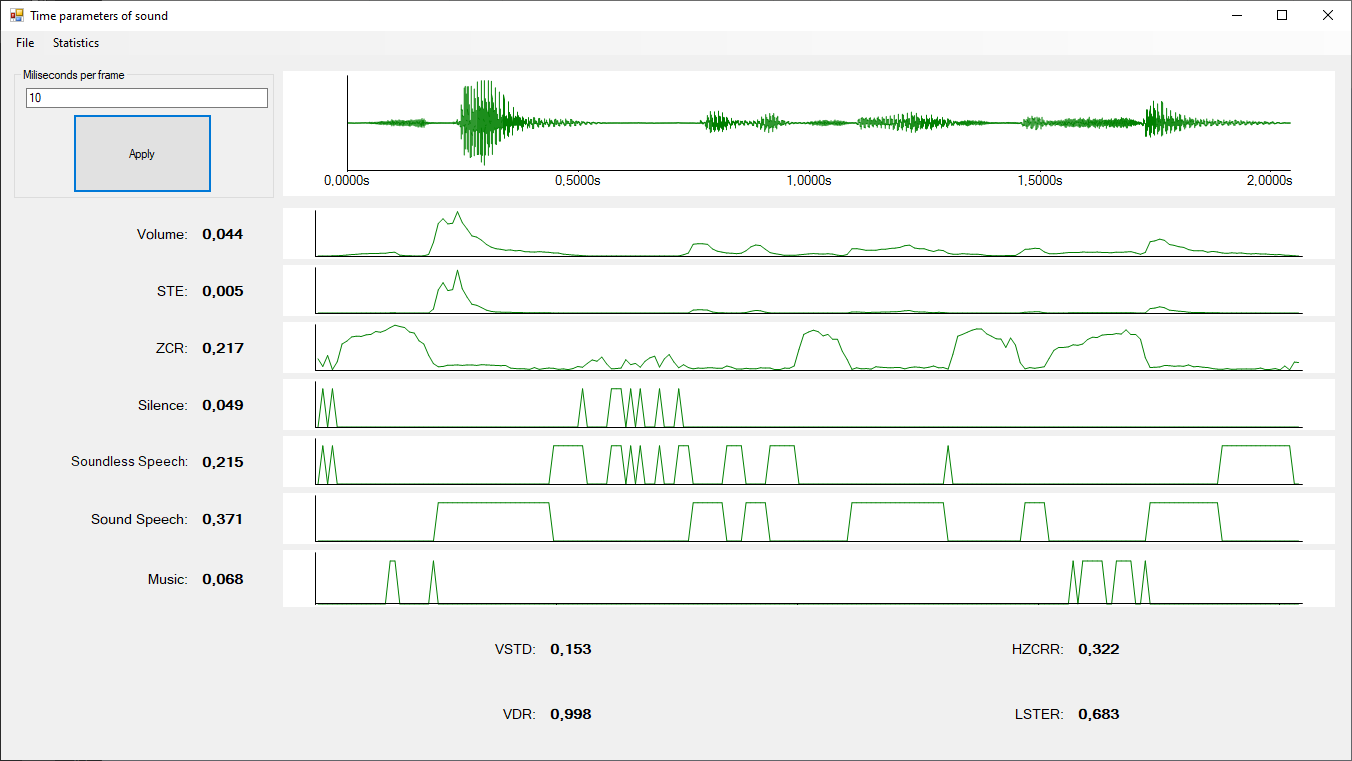
\includegraphics[width=\linewidth]{images/03normalized.png}
  \caption{Znormalizowane nagranie}
\end{figure}

\subsubsection{Głośność (Volume)}
Wartość głośności dla każdej klatki wyliczana jest zgodnie ze wzorem dostępnym w materiale źródłowym, czyli:
\begin{equation}
Volume(n) = \sqrt{\frac{1}{M} \sum_{i=0}^{M-1}s_n^2(i)}
\end{equation}
Głośność jest wartością blisko powiązaną z amplitudą fali, co widać na wszystkich powyższych rysunkach. Dotyczy to zarówno formy znormalizowanej jak i nieznormalizowanej.\\
Zgodnie z oczekiwaniami, różnice między wykresami głośności dla obu tych wariantach ograniczają się do zakresu wartości. Widać to chociażby po mniejszej wartości średniej dla nagrania znormalizowanego. Różnica ta zależy od charakterystyki mikrofonu, którą proces normalizacji ma na celu zniwelować.

\subsubsection{Energia (Short Time Energy)}
Energia dla danej ramki jest niczym innym niż wartością głośności podniesioną do kwadratu:
\begin{equation}
STE(n) = \frac{1}{M} \sum_{i=0}^{M-1}s_n^2(i) = (Volume(n))^2
\end{equation}
Wartości energii, są niższe od wartości głośności. Jest to oczywiste biorąc pod uwagę fakt iż wartość bezwzględna amplitudy dla nagrania (zarówno znormalizowanego jak i nieznormalizowanego), jest mniejsza od $1$. 

\subsubsection{Liczba przejść przez zero (Zero Crossing Rate)}
Jak sama nazwa wskazuje, współczynnik ten określa liczbę przejść amplitudy przez zero w jednej ramce sygnału. Można go określić korzystając z następującego wzoru:
\begin{equation}
ZCR(n) = \frac{1}{2M} \sum_{i=0}^{M-1}|sign(s_n(i)) - sign(s_n(i-1))|
\end{equation}
Zgodnie z oczekiwaniami - wartość ta jest jednakowa dla nagrania nieznormalizowanego i znormalizowanego.
\vspace{0.25in}\\
Powyższe współczynniki są pomocne przy określaniu również innych parametrów dźwięku.\\
W przypadku kolejnych trzech parametrów, obliczenia opierają się na klasyfikacji danej ramki ze względu na wartości już obliczonych parametrów i w zależności od wyniku, nadaniu określanemu parametrowi wartości $0$ lub $1$.

\subsubsection{Cisza (Silent Ratio)}
Miara określana na podstawie głośności i ZCR. Ramki o dostatecznie małych wartościach tych parametrów, można zaklasyfikować jako ciszę. W przypadku tego projektu, wartościami granicznymi okazały się $0.005$ dla głośności oraz $0.1$ dla ZCR.

\subsubsection{Mowa bezdźwięczna (Soundless Speech)}
Miara określana na podstawie energii i ZCR. Aby ramka została zaklasyfikowana jako zawierająca mowę bezdźwięczną, energia oraz ZCR muszą być dostatecznie małe. Jest to zatem parametr określany podobnie do ciszy, w tym przypadku jednak należy zastosować inne progi.\\
Energia (która odróżnia mowę bezdźwięczną od ciszy) nie powinna przekraczać $0.001$. Próg dla ZCR pozostaje niezmieniony i równy $0.1$.

\subsubsection{Mowa dźwięczna (Sound Speech)}
Określanie tej miary jest analogiczne do mowy bezdźwięcznej. Jedyną różnicą jest fakt iż mowa dźwięczna przenosi większą energię niż bezdźwięczna - stąd też w tym przypadku wartość energii powinna przekraczać określoną granicę $0.001$.

\subsubsection{Muzyka (Music)}
Istnieje wiele sposobów detekcji muzyki w nagraniu audio. Określanie jej na podstawie wyliczonych w tym projekcie parametrów jest możliwe, jednak obarczone dużym błędem. Zgodnie z koncepcją przedstawioną w opracowaniu dostępnym pod adresem \url{https://www.sciencedirect.com/science/article/pii/S101836391830850X}, muzyka różni się od mowy dźwięcznej wyższą wartością parametru ZCR. W przypadku tego projektu, za muzykę uznane są klatki dla których energia przekracza $0.001$ a ZCR przekracza $0.1$.\\

\subsection{Cechy na poziomie klipu (Clip-level)}
Określanie cech na poziomie ramki nie może dostarczyć wszystkich informacji - bierze ono pod uwagę krótki wycinek (ramkę) pliku audio. Dlatego też ogólna charakterystyka nagrania musi być opisywana innymi parametrami. Służą do tego parametry określane na poziomie klipu, wyliczane z użyciem opisanych powyżej parametrów Frame-level. W tej sekcji zostały opisane wszystkie cechy określane w projekcie, jednak można ich zdefiniować znacznie więcej.

\subsubsection{Znormalizowane odchylenie standardowe głośności (Volume Standard Deviation - VSTD)}
Normalizacja zawarta w nazwie tego parametru polega na podzieleniu odchylenia standardowego głośności przez maksymalną głośność w klipie. Wartość parametru jest zatem dana wzorem:
\begin{equation}
VSTD = \frac{1}{Volume_{max}}\sqrt{\frac{\sum_{n=0}^{N-1}(Volume(n)-Volume_{avg})^2}{N}}.
\end{equation}
W powyższym wzorze \textit{$N$} oznacza liczbę ramek w nagraniu, \textit{$Volume_{max}$} to najwyższa wartość głośności w nagraniu zaś \textit{$Volume_{avg}$} to średnia wartość głośności w nagraniu.

\subsubsection{Rozpiętość tonalna (Volume Dynamic Range - VDR)}
Różnica między najcichszym i najgłośniejszym fragmentem nagrania. 
\begin{equation}
VDR = \frac{Volume_{max} - Volume_{min}}{Volume_{max}}
\end{equation}
Dzięki normalizacji różnicy głośności przez wartość maksymalną, wartość VDR zazwyczaj jest zbliżona do 1. W przypadku sygnałów ciągłych o stałej wartości, zbliżona jest do 0.

\subsubsection{High Zero Crossing Rate Ratio (HZCRR)}
Jest to jeden ze współczynników bazujących na ZCR, pozwalających odróżnić nagranie zawierające muzykę od zawierającego mowę. Jego wartość obliczana jest według wzoru:
\begin{equation}
HZCRR = \frac{1}{2N}\sum_{n=0}^{N-1}[sign(ZCR(n)-1.5*avg_{ZCR})+1]
\end{equation}
Symbol $avg_{ZCR}$ w powyższym wzorze oznacza średnią wartość ZCR w 1-sekundowym oknie (a więc $avg_{ZCR}$ jest dla danego nagrania niezależne od zadanej długości ramki).

\subsubsection{Low Short Time Energy Ratio (LSTER)}
Odsetek liczby ramek w których STE są mniejsze niż 50\% średniej energii w 1-sekundowym oknie. 
\begin{equation}
LSTER = \frac{1}{2N}\sum_{n=0}^{N-1}[sign(0.5*avg_{STE}-STE(n))+1]
\end{equation}
Symbol $avg_{STE}$ oznacza średnią wartość energii w oknie 1-sekundowym.\\
Wartość współczynnika LSTER dla mowy jest zazwyczaj znacznie wyższa niż dla muzyki co pozwala z dużą skutecznością odróżnić muzykę od mowy.

\section{Wyniki działania}
Szczególnie istotnymi aspektami projektu, na których warto się skupić jest odróżnianie muzyki od mowy (oraz podział mowy na dźwięczną i bezdźwięczną).\\
W tym celu już na etapie implementacji należało poświęcić dużo czasu na odpowiednie dobranie parametrów granicznej głośności, energii czy liczby przejść przez zero. W tym celu posiłkowano się dostępnymi już programami i starano się dostosować wyniki zwracane przez tworzony program do rezultatów poprawnych. Należy jednak pamiętać, że równie ważne (albo i ważniejsze) jest zachowanie zdrowego rozsądku - odróżnienie muzyki od mowy za pomocą słuchu jest prostsze i efektywniejsze.\\
Testowymi nagraniami były już wspomniane nagrania korpusu tekstowego, jednak z powodu braku muzyki analizie zostały poddane również inne pliki źródłowe.
\subsection{Mowa z podkładem muzycznym}
Przykładem jest już wspomniany utwór \textit{Portier!} Taco Hemingwaya. Na poniższych zdjęciach fragment rozmowy z muzyką w tle (\textit{Rysunek 4}) oraz samej narastającej muzyki (\textit{Rysunek 5}).
\begin{figure}[H]
  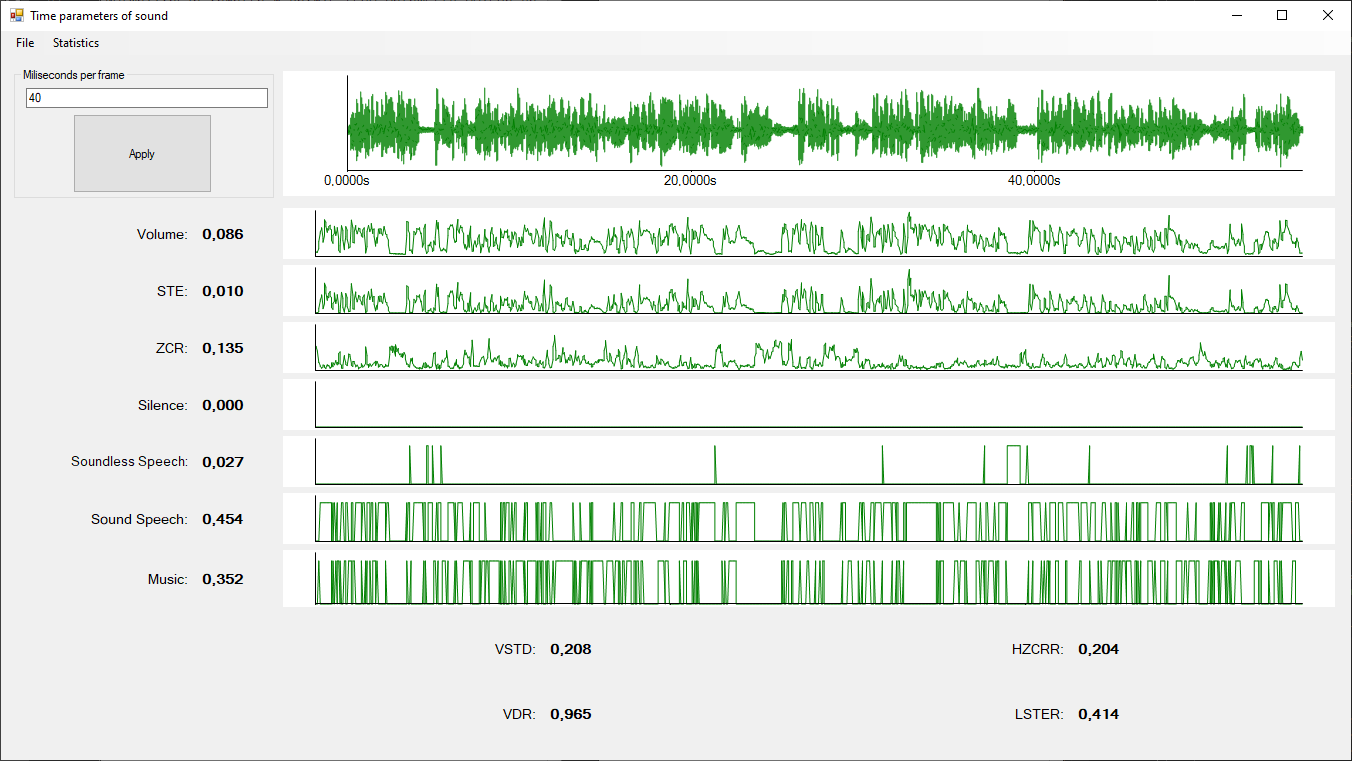
\includegraphics[width=\linewidth]{images/04speech.png}
  \caption{Fragment rozmowy z utworu \textit{Portier!} Taco Hemingwaya}
\end{figure}
\begin{figure}[H]
  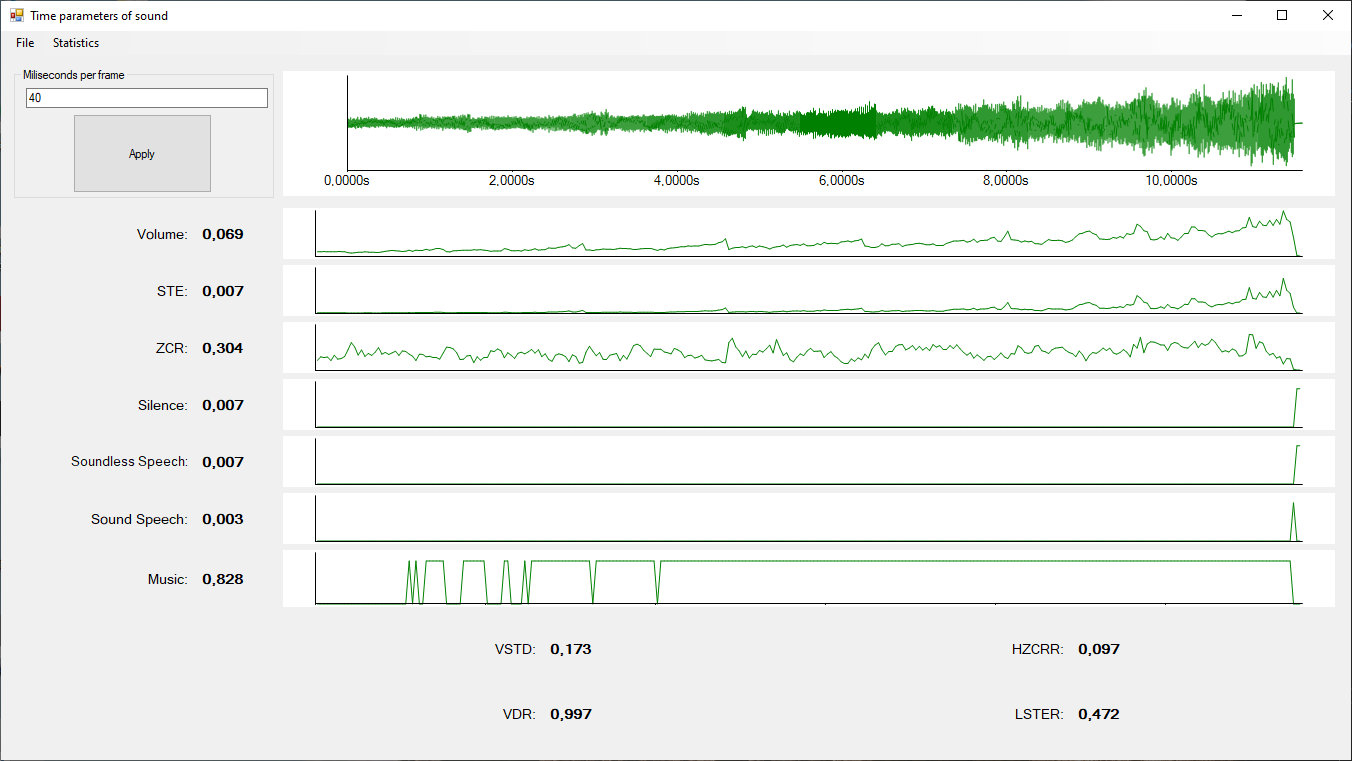
\includegraphics[width=\linewidth]{images/05music.png}
  \caption{Fragment muzyki z utworu \textit{Portier!} Taco Hemingwaya}
\end{figure}
Jak widać na tym przykładzie, parametry Frame-level okazały się zawodne, a muzyka będąca podkładem do słów wyraźnie wybijała się w trakcie nagrania rozmowy. Niestety oznacza to, iż ciężko wyciągnąć wnioski analizując utwory zawierające mowę przeplataną z muzyką.\\
Potwierdzać zdają się to parametry Clip-level. Przykładowo LSTER, który powinien być dla mowy znacznie wyższy, jest niewiele niższy.
\subsection{Mowa a muzyka}
Sytuacja prezentuje się inaczej przy osobnej analizie nagrania mowy oraz muzyki. W tym celu powołam się ponownie na zapowiedziany we wstępie fragment przemówienia Baracka Obamy (\textit{Rysunek 6}) oraz utwór instrumentalny (\textit{Rysunek 7}).
\begin{figure}[H]
  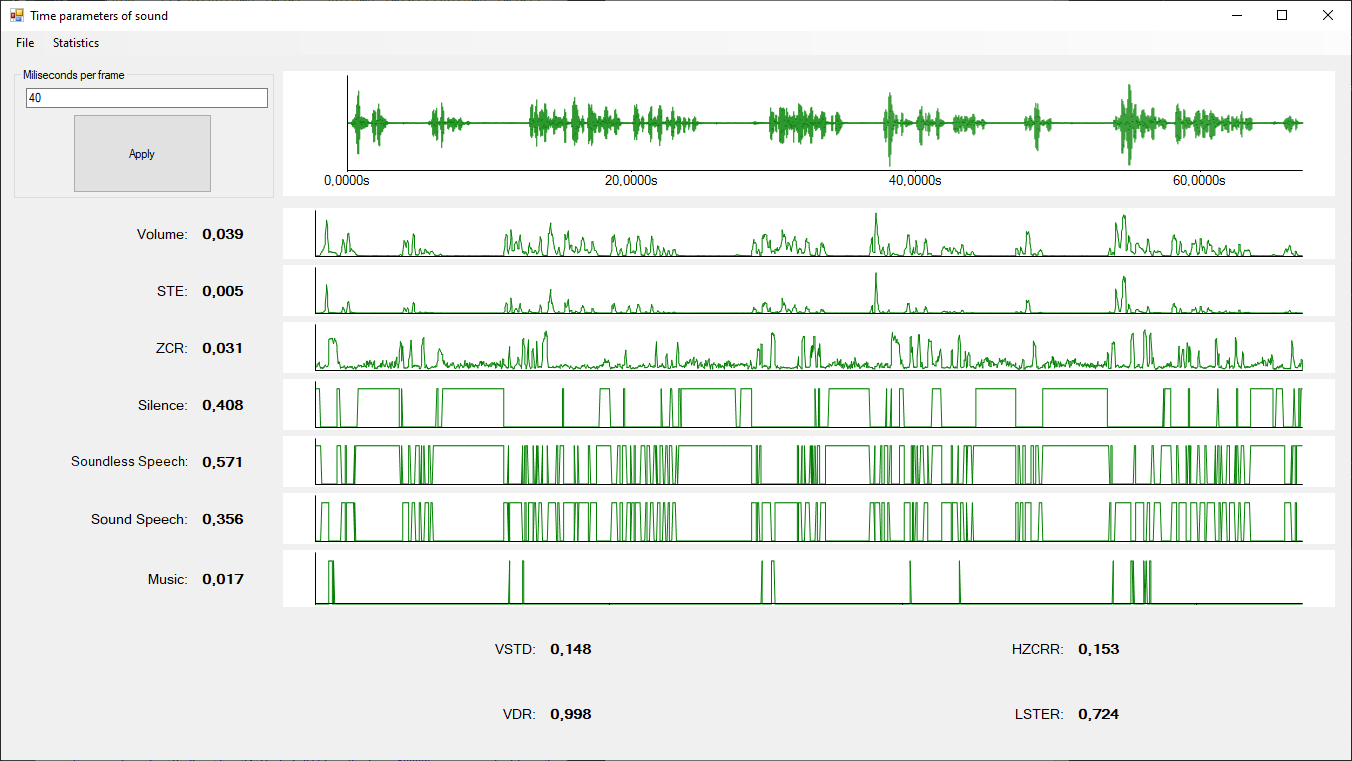
\includegraphics[width=\linewidth]{images/06sampleSpeech.png}
  \caption{Fragment przemówienia Baracka Obamy}
\end{figure}
\begin{figure}[H]
  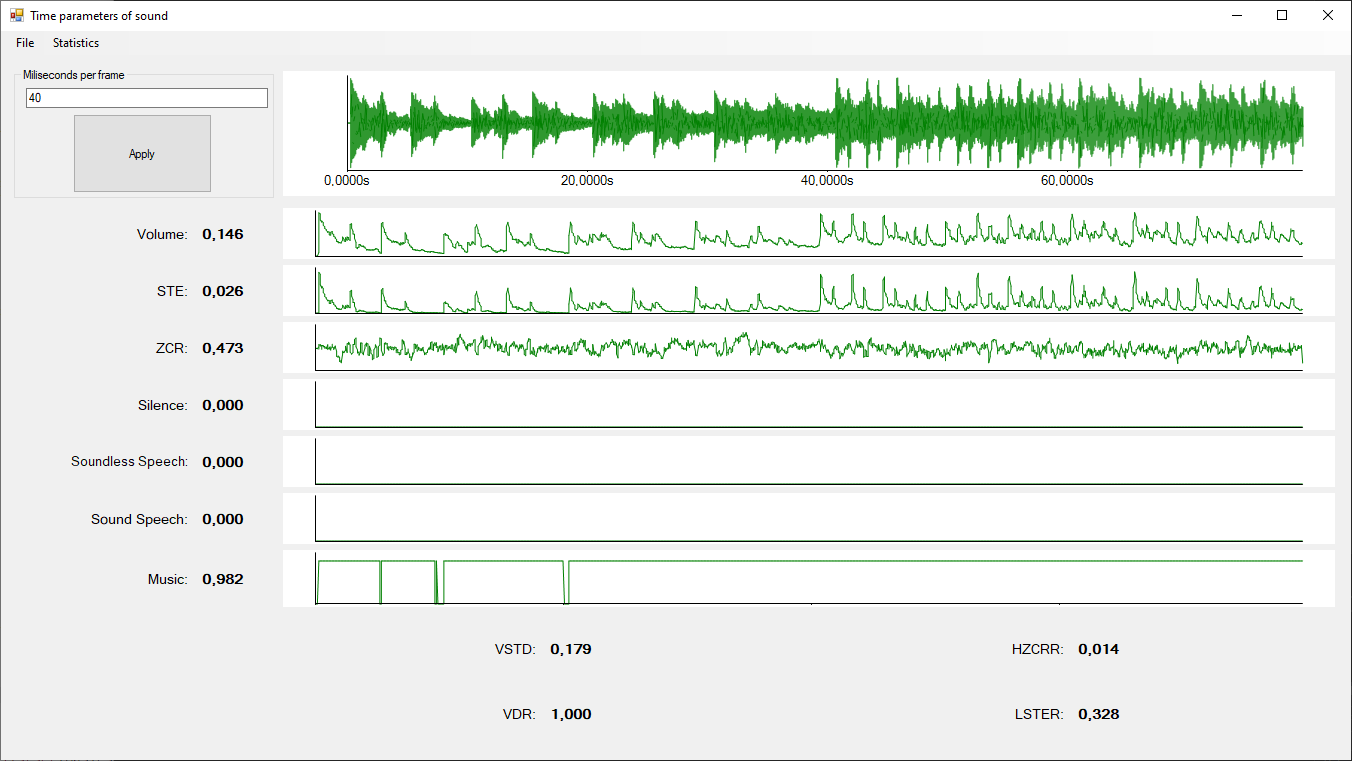
\includegraphics[width=\linewidth]{images/07sampleMusic.png}
  \caption{Fragment muzyki z utworu \textit{Adventure} stworzonego przez Bensound}
\end{figure}
Jak widać, w przypadku przemówienia ilość wykrytej muzyki jest niewielka, w szczególności w porównaniu z mową. Znaczna część przemówienia określona jest jednak jako cisza. Absolutnie nie jest to jednak błędem! Wystarczy spojrzeć na wykres amplitudy wczytanego nagrania na którym znajduje się bardzo dużo przerw, co można potwierdzić odsłuchując faktyczne przemówienie.\\
Natomiast dla utworu instrumentalnego, ilość ciszy oraz mowy jest zerowa, mimo występowania fragmentów o niskiej głośności czy energii. Ponadto niemal cały utwór został zaklasyfikowany jako muzyka, co pozwala wysoko ocenić skuteczność parametrów Frame-level.\\
Dodatkowo wartość LSTER również pokrywa się z oczekiwaniami - wartość $0.724$ dla przemówienia może zostać spokojnie zaklasyfikowana jako dużo wyższa niż $0.328$ dla muzyki.

\section{Wnioski}
Parametry określane przez program są wystarczająco dokładne aby odróżnić nagranie muzyki od nagrania mowy. Jednak jeśli występują one jednocześnie, dokładność nie pozwala na określenie przedziałów gdzie muzyka/mowa dominuje.

\lstset{basicstyle=\ttfamily}
\lstset{style=sharpc}
\begin{lstlisting}
\end{lstlisting}

\end{document}